\documentclass[12pt,a4]{article}
\usepackage[left=1.8cm,right=1.8cm,top=32mm,columnsep=20pt]{geometry}

\usepackage[utf8]{inputenc} %Formato de codificación
\usepackage[spanish, es-tabla, es-nodecimaldot]{babel}
\usepackage{amsmath} %paquete para escribir ecuaciones matemáticas
\usepackage{float} %Para posicionar figuras
\usepackage{graphicx} %Para poder poner figuras
\usepackage{tikz}
\usetikzlibrary{positioning}
\usetikzlibrary{shapes.geometric, decorations.pathreplacing}

\title{Analisis movimiento de un pendulo}
\author{Francisco Carruthers, Facundo Firpo y Joel Jablonski\\ [2mm]
\small \texttt{\{fcarruthers, ffirpo, jjablonski\}@udesa.edu.ar}\\
\small Fisica I, tutorial Vinograd}
\date{2do Semestre 2024}


\begin{document}

\maketitle

\begin{abstract}
    Pendulo
\end{abstract}

\section{Introduccion}


\section{Practica experimental}


\section{Seguimiento de la trayectoria}


\section{Resultados}

\begin{figure}[H]
    \centering
    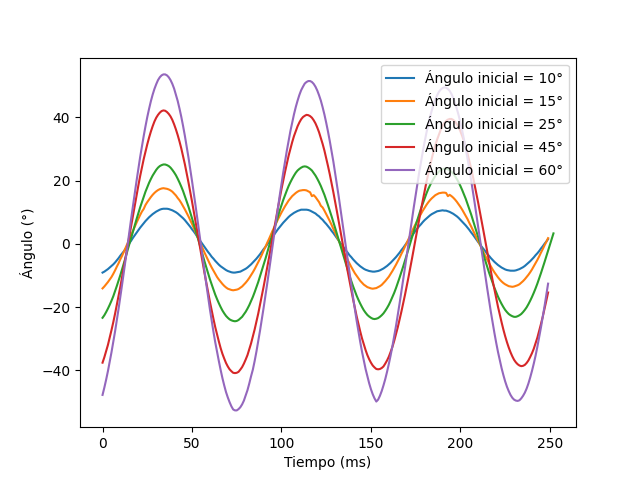
\includegraphics[width=0.6\linewidth]{angulos.png}
    \caption{Posicion de la masa en funcion del tiempo para distintos angulos iniciales}
    \label{fig:angulos}
\end{figure}

Se puede observar como la amplitud del movimiento no afecta la frecuencia del mismo.

\begin{figure}[H]
    \centering
    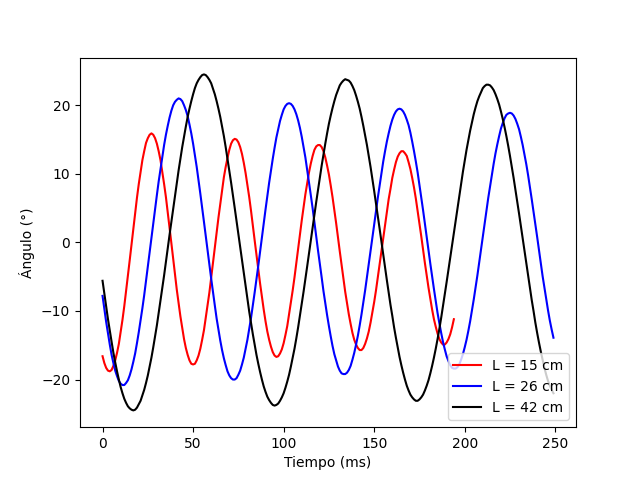
\includegraphics[width=0.6\linewidth]{largo.png}
    \caption{Posicion de la masa en funcion del tiempo para distintos largos de soga}
    \label{fig:largo}
\end{figure}

Se puede observar como el largo de la soga afecta la frecuencia del movimiento. A mayor largo, menor frecuencia. Esto se debe a que la bolita recorre una mayor distancia. Sabemos que la longitud de arco esta defenida como $d = r \theta$, por lo que a mayor longitud de soga, mayor longitud de arco recorre la bolita.

\begin{figure}[H]
    \centering
    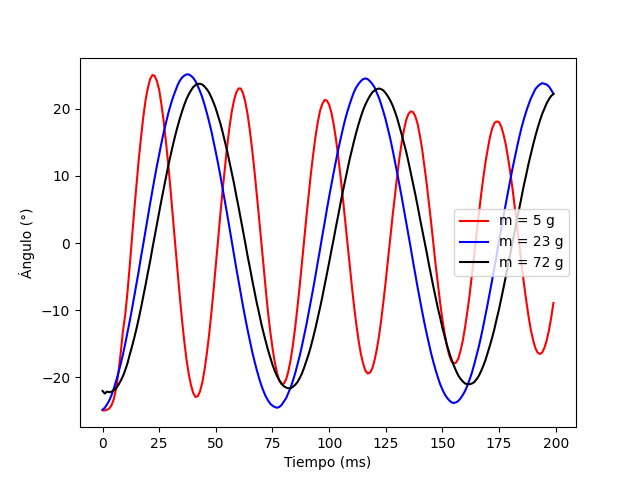
\includegraphics[width=0.6\linewidth]{peso.png}
    \caption{Posicion de la masa en funcion del tiempo para distintas masas}
    \label{fig:masa}
\end{figure}

Se puede observar como la masa de la bolita tambien afecta la frecuencia del movimiento. Esto se debe a que a mayor masa, mayor peso ya que esta dado por $p = m \cdot \vec{g}$.

\end{document}